%% Dokumenteinstellungen
\documentclass{template}

% Basierend auf der Vorlage des MNM-Teams
% - optimiert für die Arbeit mit gängigen LaTeX-Editoren
% - funktioniert ohne Makefile und Anpassungen der LaTeX-Verzeichnisstruktur
% - verwendet Komaskript für ein (nach europäischen Gepflogenheiten) schöneres Layout
%
% Copyright: CC BY-NC 4.0
% Verbesserungen werden gerne übernommen, wenn sie den Autoren bekannt gemacht werden
%
% v1, 2007 (Michael Brenner)
% v1.1, 2012 (Michael Brenner)
% v1.2, 2017 (Michael Brenner)
% v1.2.1, 2017 (Benjamin Schnoy)
% v1.3, 2018 (Michael Grabatin)
% v1.4, 2022 (Daniela Pöhn)
% v1.4.1, 2022 (Daniela Pöhn)
% v1.4.2, 2023 (Mark Minas)

%
% der Befehl \hypenation versteht keine Sonderzeichen, also weder ä
% noch "a noch \"a. Wörter die derartige Zeichen enthalten müssen
% direkt im Text getrennt werden, z.B. Wör\-ter
%
\hyphenation{Ba-che-lor-ar-beit}
\hyphenation{Ma-ster-ar-beit}
\hyphenation{Ma-nage-ment}
\hyphenation{Ma-nage-ment-agent}
\hyphenation{Ma-nage-ment-agent-en}
\hyphenation{Ma-nage-ment-ar-chi-tek-tur}
\hyphenation{Ma-nage-ment-ar-chi-tek-tu-ren}
\hyphenation{Ma-nage-ment-an-wen-dung}
\hyphenation{Ma-nage-ment-an-wen-dung-en}
\hyphenation{Ma-nage-ment-an-for-der-ung}
\hyphenation{Ma-nage-ment-funk-ti-on}
\hyphenation{Ma-nage-ment-funk-ti-onen}
\hyphenation{Ma-nage-ment-kon-zep-te}
\hyphenation{Ma-nage-ment-res-source}
\hyphenation{Ma-nage-ment-in-for-ma-ti-on}
\hyphenation{Ma-nage-ment-res-sour-cen}
\hyphenation{ma-nage-ment-re-le-vante}
\hyphenation{ma-nage-ment-sy-stem}
\hyphenation{ma-nage-ment-sy-steme}
\hyphenation{Ma-nage-ment-in-stru-men-tie-rung}
\hyphenation{Ma-nage-ment-platt-form}
\hyphenation{Sys-te-men}
\hyphenation{Sys-tem-um-ge-bun-gen}
\hyphenation{Sys-tem-ma-nage-ment}
\hyphenation{DHCP}
\hyphenation{Ma-nage-ment-diszi-plinen}
\hyphenation{System-management-architekturen}
\hyphenation{Verwendungs-nachweise}
\hyphenation{Video-einricht-ungen}
\hyphenation{Res-source}
\hyphenation{Res-sourcen}
\hyphenation{Grund-anwendung}
\hyphenation{Grund-anwendungen}
\hyphenation{Basis-anwendung}
\hyphenation{Core}
\hyphenation{Kom-mu-ni-ka-ti-on}
\hyphenation{De-sign-ent-schei-dung}
\hyphenation{Sprung-ad-res-sen}
\hyphenation{Klas-si-fi-ka-ti-on}
\hyphenation{Schreib-recht}
\hyphenation{Be-nut-zer-zer-ti-fi-kat}
\hyphenation{Bau-stein-ent-wi-ckler}
\hyphenation{ad-mi-ni-stra-ti-ve}

 % in dieses File kommen Wörter, die Latex nicht richtig trennt

% Genau eine der beiden folgenden Optionen muss gewählt werden. 
% Wenn man twoside=true wählt, aber nur einseitig druckt, befinden sich
% die Seitennummern bei geraden Seiten auf der falschen Seite, und es
% können leere Seiten am Ende eines Kapitels entstehen.
\KOMAoptions{twoside=true}  % bei doppelseitigem Druck
%\KOMAoptions{twoside=false} % bei einseitigem Druck

\pagenumbering{roman} % damit im Frontmatter keine arabischen Seitenzahlen erscheinen

% Hier können weitere Pakete hinzugefügt werden

\begin{document}

%%%% Einfacheres Ausfüllen der Titelseite
\newcommand{\Dname}{Vorname Nachname} % Hier den Namen des Bearbeiters eintragen
\newcommand{\Dnummer}{Matrikelnummer} % Hier die Matrikelnummer eintragen
\newcommand{\Dtitel}{Titel der Arbeit} % Hier den Titel eintragen. Ggf. muss dieser getrennt werden
\newcommand{\Darbeit}{Bachelorarbeit,Masterarbeit} % Hier die Art der Abschlussarbeit eintragen
\newcommand{\Dprofa}{Prof. Dr. Wolfgang Hommel} % Hier den Aufgabensteller eintragen
\newcommand{\Dprofb}{Prof. Dr. Zweiter Prüfer} % Hier den Zweitprüfer eintragen
\newcommand{\Dbetreuera}{Betreuer 1} % Hier den Betreuer 1 eintragen
\newcommand{\Dbetreuerb}{Betreuer 2} % Hier den Betreuer 2 eintragen (meist alphabetisch). Falls nicht vorhanden, leer lassen. Ggf. auf der Titelseite löschen.
\newcommand{\Dbetreuerc}{Externer Betreuer} % Hier den Betreuer 3  bzw. externen Betreuer eintragen. Falls nicht vorhanden, leer lassen. Ggf. auf der Titelseite löschen.
\newcommand{\Dday}{01.01.2022} % Hier das Abgabedatum eintragen
\newcommand{\Dversion}{Draft vom \today} % Wenn kein Draft mehr, sondern Endversion, dann ``Draft vom \today'' löschen

% ---------------------------------------------------------------
\frontmatter
% ---------------------------------------------------------------
\mainmatter % die eigentliche Arbeit

\chapter{Einleitung}
\label{sec:einleitung}

Einleitender Text

\section{Motivation}

Beschreibung der Motivation, siehe Abbildung~\ref{fig:LampFlowchart}.

%Grafik aus PNG-File - bei dieser Variante darauf achten, dass die Grafik in ausreichender Auflösung vorliegt (so dass auch nach Skalierung >300dpi im Ausdruck erreicht werden)
\begin{figure}[htb]
  \centering
  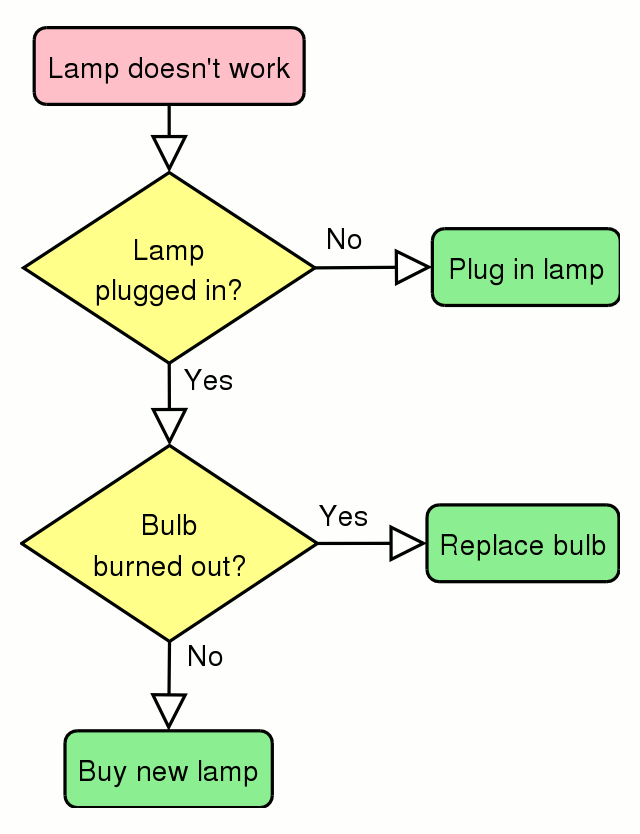
\includegraphics[width=.4\textwidth]{LampFlowchart}\\ % PNG-File
  \caption{Nulla interdum aliquam leo}\label{fig:LampFlowchart}
\end{figure}


\section{Ziele der Arbeit}

Ziele der Arbeit (vgl. Abbildung~\ref{fig:BurgerFlowchart}). Als Bonus können auch Forschungsfragen formuliert werden.

%Grafik aus PDF-File - diese Variante ist vorzuziehen, da sie die Einbundung echter Vektorgrafiken ermöglicht
\begin{figure}[htb]
  \centering
  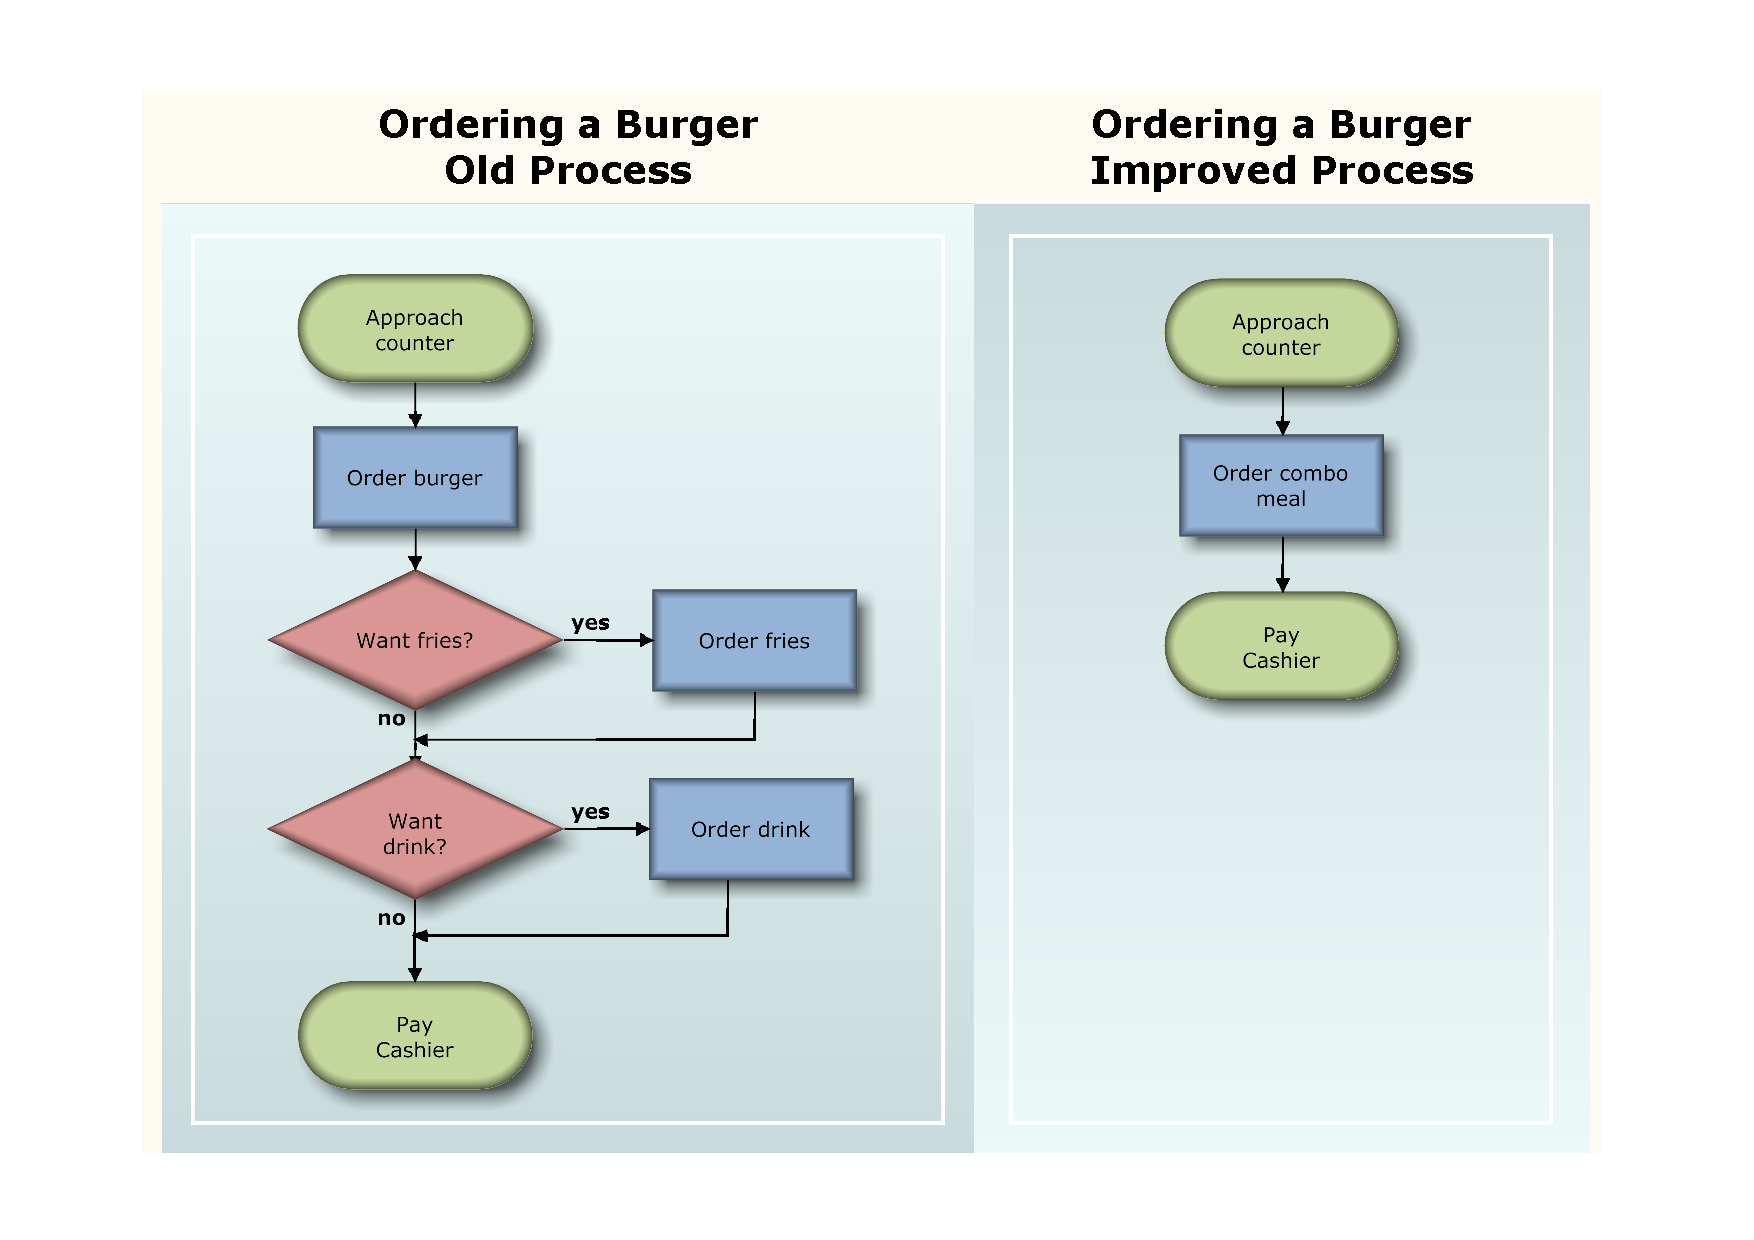
\includegraphics[scale=.6]{BurgerFlowchart}\\ % PDF-File
  \caption{Donec tempor leo a massa~\cite{praxisbuch2017} (Zitat aus Norm, Handbuch u.ö.)}\label{fig:BurgerFlowchart}
\end{figure}

Quisque ligula orci, accumsan vel, molestie ac, lacinia non, lorem . Fusce nonummy. Cras mattis, elit ac tempor congue, ante arcu porta justo, at rhoncus sapien erat vel dui~\cite{latexbib}. Phasellus vestibulum, turpis non tempor vehicula, quam lacus accumsan dolor, id dictum magna magna eu neque. Sed suscipit placerat odio. Sed et sem. Mauris vel tortor a nisl egestas vulputate. Aliquam facilisis luctus nibh. Maecenas vel lectus sed urna viverra pretium. Aenean malesuada nibh sed ipsum. Fusce vel augue. Mauris eget massa. Class aptent taciti sociosqu ad litora torquent per conubia nostra, per inceptos hymenaeos. Etiam nec justo eu purus ultricies mattis. In leo ante, adipiscing sit amet, ultrices at, ultrices et, nulla. Mauris quis odio. Donec sollicitudin rutrum sapien. Aliquam eget ante a dui euismod porttitor. Donec commodo scelerisque purus. Sed magna.\ac{DFN}

\section{Vorgehen und Aufbau}

Der Aufbau der Arbeit ausformuliert.

Nullam consectetuer risus vitae orci. Aliquam fermentum leo sit amet nulla laoreet hendrerit. Maecenas tempus, neque eu posuere vestibulum, pede eros adipiscing augue, pulvinar ullamcorper lectus lectus et tellus. Donec at velit at velit pellentesque sagittis. Vestibulum ultricies ultrices mi. Vestibulum accumsan dictum ligula. Ut lobortis, odio ut semper vehicula, nibh quam semper nisi, sed adipiscing purus lectus et sem. Mauris nisl est, scelerisque ut, ultrices nec, faucibus vitae, nulla. Nulla nisi. Suspendisse potenti. Etiam ultrices commodo odio. Quisque turpis purus, mollis sed, pretium quis, volutpat et, neque. Nam a sapien eget neque consectetuer ornare. Pellentesque felis metus, pellentesque quis, volutpat rhoncus, laoreet id, nunc. Duis egestas, felis et luctus vestibulum, velit nunc luctus felis, non tempor justo ligula et nulla. Vestibulum, Abbildung~\ref{fig:tabelle}, est. Nulla aliquam eleifend justo.


\begin{table}[htb]
  \centering
  \begin{tabular}{|l|c|}
    \hline
    \textbf{tempus} & \textbf{risus} \\ \hline
    ultrices & pellentesque \\
    rhoncus & egestas \\
    \hline
  \end{tabular}
  \caption{Aliquam fermentum}\label{fig:tabelle}
\end{table}

\endinput
 % Als erstes kommt eine Einleitung.
\chapter{Grundlagen}
\label{sec:grundlagen}

Hier werden die Grundlagen zum Thema beschrieben. Was muss eine Kommilitonin oder ein Kommilitone noch wissen, damit sie oder er mein Thema versteht?
 % Das Grundlagenkapitel je nach Menge und Thema auch auf zwei Kapitel aufgeteilt sein.
\chapter{Anforderungsanalyse}
\label{sec:anforderungsanalyse}

Um wissenschaftlich korrekt zu erfassen, was konzipiert und umgesetzt werden soll, werden Anforderungen erstellt. Am einfachsten ist dies anhand verschiedener Szenarien, die den Ist-Zustand beschreiben. Um zum Soll-Zustand zu gelangen, müssen bestimmte Anforderungen, die Sie aufstellen, erfüllt werden. Durch die Verwendung mehrerer Szenarien sind diese Anforderungen nicht auf ein bestimmtes Szenario zugeschnitten, sondern möglichst allgemeingültig. Andere Varianten sind eine allgemeine Herleitung und basierend auf Literatur.

Je nachdem wie viele Anforderungen Sie aufstellen, kann es notwendig sein, diese zu gruppieren (z.B. funktionale und nicht-funktionale Anforderungen) und/oder zu gewichten (z.B. MUSS, SOLL, KANN). Praktisch ist eine Anforderungstabelle am Ende des Kapitels, welche alle Anforderungen gesammelt zeigt. Diese Tabelle lässt sich leicht weiterverwenden.

Im nächsten Kapitel vergleichen Sie die aufgestellten Anforderungen mit der Literatur. Diese kann einzelne Anforderungen vollständig, teilweise oder gar nicht erfüllen. Das herausgearbeitete Delta begründet Ihre Arbeit. Abschließend müssen die Anforderungen mit der eigenen Lösung im Kapitel Evaluation verglichen werden.
 % Die Anforderungsanalyse je nachdem auch an einer anderen Stelle stehen. Nur in den wenigsten Fällen benötigt man keine.
\chapter{Stand von Forschung und Technik}
\label{sec:literaturrecherche}

Lösen wissenschaftliche (und praktische) Ansätze die wissenschaftliche Fragestellung gar nicht oder teilweise? In diesem Kapitel werden Ansätze vorgestellt, deren Vor-und Nachteile u.a. basierend auf den aufgestellten Anforderungen diskutiert.
 % Der Vergleich der Literatur mit den aufgestellten Anforderungen begründet die eigene Arbeit.
\chapter{Konzept}
\label{sec:konzept}

Der eigentliche Hauptteil
 % Anschließend wird der Hauptteil beschrieben. Bei einer Implementierung wird zunächst die Architektur beschrieben. Bei einer Studie wird erst das Studiendesign erklärt.
\chapter{Umsetzung}
\label{sec:umsetzung}

Tragfähigkeitsnachweis des Hauptteils, wie z.B. in Form einer Implementierung.
 % Basierend darauf folgt die Umsetzung, z.B. die Implementierung der Architektur oder die Durchführung und Ergebnisse einer Studie.
\chapter{Evaluation}
\label{sec:evaluation}

Evaluation der eigenen Lösung u.a. basierend auf den aufgestellten Anforderungen. Was wurde umgesetzt, was nicht? Wieso? Was kann verbessert werden?
 % Kann in manchen Fällen auch wegfallen
\chapter{Fazit und Ausblick}
\label{sec:fazit}

Zusammenfassung der Arbeit und Ausblick auf weiterführende Arbeiten.

\section{Zusammenfassung}

\section{Ausblick}
 % Als letztes steht eine Zusammenfassung, ein Fazit und ein Ausblick.
    % usw.

% ---------------------------------------------------------------
\backmatter 

\end{document}
